\section{The Perceptron Algorithm and its Variants}\label{sec:q4}

For this question, you will experiment with the Perceptron algorithm
and some variants on a data set.


\subsection{What to report}

\begin{enumerate}
\item~[8 points] Briefly describe the design decisions that you have
  made in your implementation. (E.g, what programming language, how do
  you represent the vectors, etc.)\\\\
  Used Python to code. Represented weight vectors using the python list. Such that position 0 of the weight vector represents the bias. Reading the input sparse matrix data into dictionaries and using this to do dot products.\\
  I have each variant of the perceptron as a separate class and creating an object of any variant takes in data and the max variable in the data.\\
  Calling a run perceptron on the object trains the perceptron and returns a weight vector.\\
  Pseudo random data read for training the classifier with a seed of 6 used.
\item~[2 points] {\em Majority baseline:} Consider a classifier that
  always predicts the most frequent label. What is its accuracy on
  test and development set?\\
  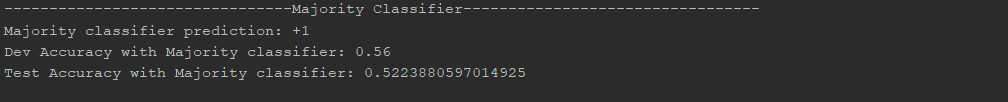
\includegraphics[width=\textwidth]{maj_class.PNG}\\
  Test Accuracy: 52.24\%\\
  Dev Accuracy: 56\%
\item~[10 points per variant] For each variant above (5 for 6350 students, 4 for 5350 students), you need to report:\\
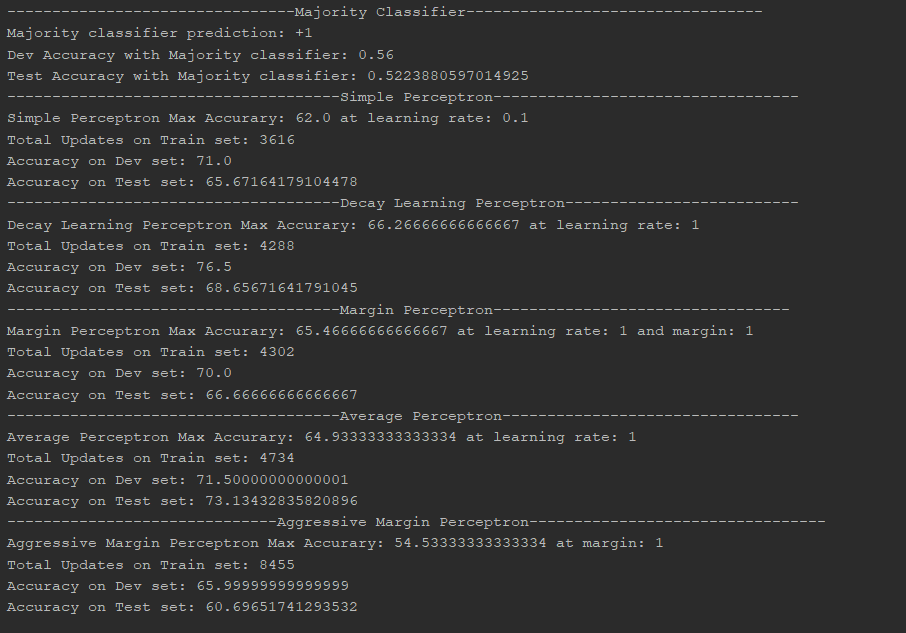
\includegraphics[width=\textwidth]{accuracies.PNG}\\
  \begin{enumerate}
  \item The best hyper-parameters

  \item The cross-validation accuracy for the best hyperparameter 
    \begin{itemize}
      \item Simple Perceptron: Learning rate = 0.1; Accuracy = 62\%
      \item Decay Learning Perceptron: Learning rate = 1; Accuracy = 66.27\%
      \item Margin Perceptron: Learning rate = 1, Margin = 1; Accuracy = 65.47\%
      \item Average Perceptron: Learning rate = 1; Accuracy = 64.93\%
      \item Aggressive Margin Perceptron: Margin = 1; Accuracy = 54.53\%
  \end{itemize}
  \item The total number of updates the learning algorithm performs on the training set.
  Updates based on Max accuracy weight vector trained on training set and tested against dev set. Max 20 epoch.
  \begin{itemize}
      \item Simple Perceptron: 3616
      \item Decay Learning Perceptron: 4288
      \item Margin Perceptropn: 4302
      \item Average Perceptron: 4734
      \item Aggressive Perceptron: 8455
  \end{itemize}
  
  \item Development set accuracy
   Using Max accuracy weight vector trained on training set and tested against dev set. Max 20 epoch.
  \begin{itemize}
      \item Simple Perceptron: 71\%
      \item Decay Learning Perceptron: 76.5\%
      \item Margin Perceptropn: 70.0\%
      \item Average Perceptron: 71.5\%
      \item Aggressive Perceptron: 65.99\%
  \end{itemize}
  \item Test set accuracy
     Using Max accuracy weight vector trained on training set and tested against dev set. Max 20 epoch.
  \begin{itemize}
      \item Simple Perceptron: 65.67\%
      \item Decay Learning Perceptron: 68.66\%
      \item Margin Perceptropn: 66.67\%
      \item Average Perceptron: 73.13\%
      \item Aggressive Perceptron: 60.69\%
    \end{itemize}
  \item Plot a {\em learning curve} where the $x$ axis is the epoch id
    and the $y$ axis is the dev set accuracy using the classifier (or
    the averaged classifier, as appropriate) at the end of that
    epoch. Note that you should have selected the number of epochs
    using the learning curve (but no more than 20 epochs).
    \begin{itemize}
      \item Simple Perceptron:\\ 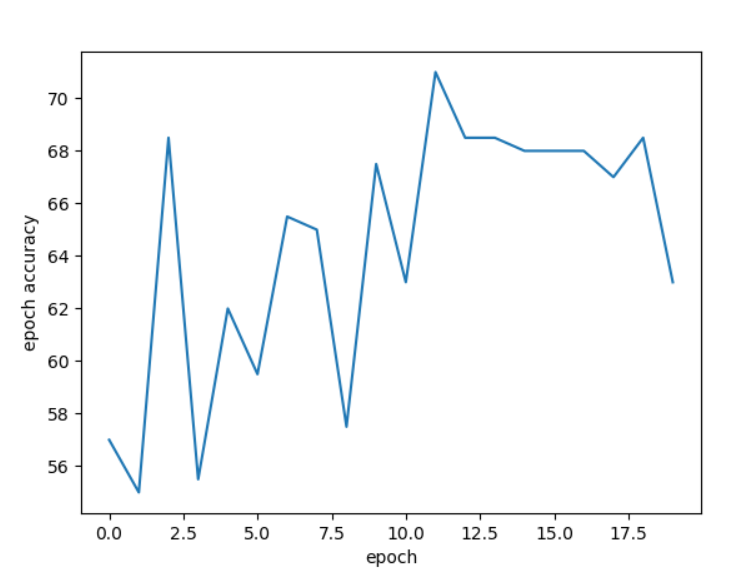
\includegraphics{simpleP.PNG}
      \item Decay Learning Perceptron:\\ 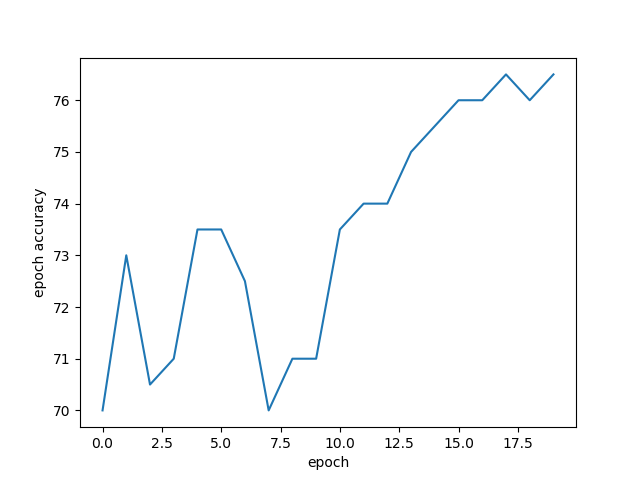
\includegraphics{decayLP.png}
      \item Margin Perceptropn:\\ 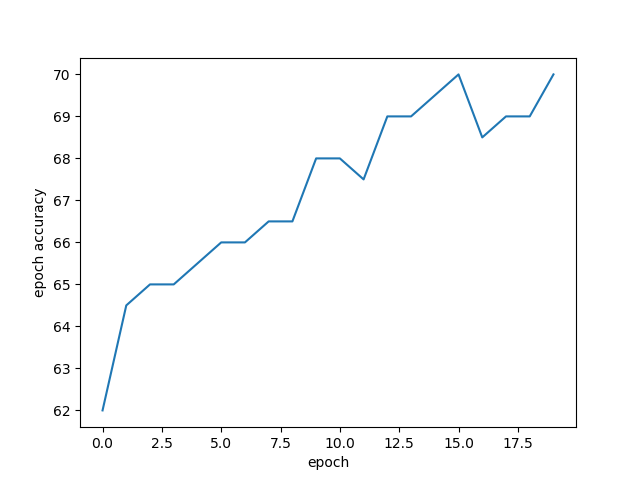
\includegraphics{marginP.png}
      \item Average Perceptron:\\ 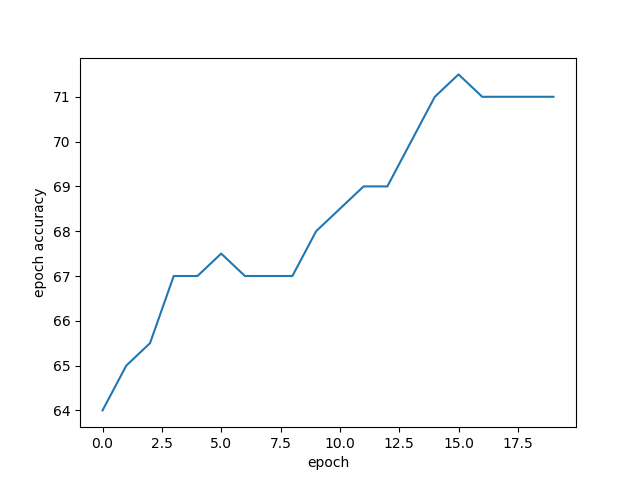
\includegraphics{avgP.png}
      \item Aggressive Perceptron:\\ 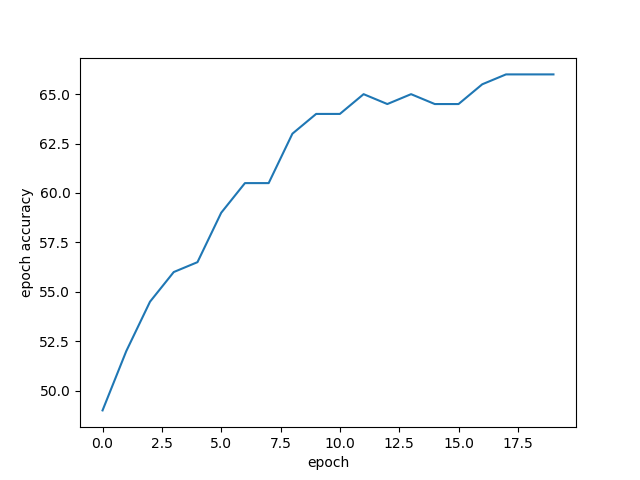
\includegraphics{aggressiveMP.png}
    \end{itemize}
  \end{enumerate}
\end{enumerate}

%%% Local Variables:
%%% mode: latex
%%% TeX-master: "hw2"
%%% End:
